%%%%%%%%%%%%%%%%%%%%%%%%%%%%%%%%%%%%%%%%%%%%%%%%%%%%%%%%%%%%%%%%%%%%%%%%%%%
% * <sonya.hanson@choderalab.org> 2015-04-23T18:56:00.248Z:
%
% 
%
% HEADER: DON'T EDIT THIS!
%%%%%%%%%%%%%%%%%%%%%%%%%%%%%%%%%%%%%%%%%%%%%%%%%%%%%%%%%%%%%%%%%%%%%%%%%%%
% ^ <sonya.hanson@choderalab.org> 2015-04-23T18:57:46.938Z.
% But why not?

\documentclass[11pt]{article}

\title{ Advancing predictive physical modeling through focused development of model systems to drive new modeling innovations}

\usepackage[top=0.5in, bottom=0.5in, left=0.5in, right=0.5in]{geometry}
\usepackage{helvet}
\usepackage{url} % hypderref?
\usepackage{graphicx}
\graphicspath{{figures/}} % The figures are in a figures/ subdirectory.
\renewcommand{\familydefault}{\sfdefault}
\pagestyle{empty}
%\pagestyle{plain}

% Fancy page-width tables
\usepackage{tabularx}

% Use a package for framed boxes
\usepackage{mdframed}

\usepackage[T1]{fontenc}
\usepackage{amssymb}


\usepackage{setspace}
\usepackage{microtype}

\usepackage{amsfonts}
\usepackage{amsmath}

\usepackage{floatrow}

\usepackage[normalem]{ulem} % for nci.bst

\usepackage{sidecap}
\usepackage[abs]{overpic}
\usepackage{wrapfig}

%\usepackage[round,authoryear]{natbib}
\usepackage{cite}
%\setlength{\bibsep}{0.00in}

\usepackage{hyperref}
\hypersetup{colorlinks=true, urlcolor=black, citecolor=black, linkcolor=black}

\newcommand{\doi}[1]{\href{http://dx.doi.org/#1}{doi:#1}}

\newcommand{\ac}[1]{{\sc \lowercase{#1}}}

\renewcommand{\baselinestretch}{.93}
%\renewcommand{\baselinestretch}{.90}
\usepackage{wrapfig} 

\usepackage{bibspacing}
\setlength{\bibspacing}{\baselineskip}


\graphicspath{{figs/}}

\makeatletter

\newcommand{\captionfonts}{\footnotesize}

\makeatletter  % Allow the use of @ in command names
\long\def\@makecaption#1#2{%
  \vskip\abovecaptionskip
  \sbox\@tempboxa{{\captionfonts #1: #2}}%
  \ifdim \wd\@tempboxa >\hsize
    {\captionfonts #1. #2\par}
  \else
    \hbox to\hsize{\hfil\box\@tempboxa\hfil}%
  \fi
  \vskip\belowcaptionskip}      
\makeatother

\renewcommand{\figurename}{{\bf Figure}}

% Page numbering.
%\pagestyle{plain}
%\pagenumbering{arabic}

\setlength{\abovecaptionskip}{-5pt}

\makeatother

\renewcommand{\refname}{Bibliography and References Cited}

\setlength{\parindent}{0pt} % Don't indent first line
%\setlength{\parskip}{1ex plus 0.5ex minus 0.2ex} % Add some space between paragraphs
\setlength{\parskip}{0.8ex} % Add some space between paragraphs

\begin{document}

%======================================
% CITE OUR REFS FIRST
%\phantom{
%\cite{mobley-chodera-dill:2006:jcp:orientation-restraints,mobley-chodera-dill:2007:jctc:confine-and-release,shirts-mobley-chodera-pande:2007:jpcb:dispersion-corrections,chodera:jcp:2007,shirts-mobley-chodera:2007:annu-rep-comput-chem:prime-time,shirts-chodera:jcp:2008:mbar,ncmc,chodera-shirts:jcp:2011:gibbs,chodera:curr-opin-struct-biol:2011:drug-discovery,chodera-shirts:jcamd:2013:yank}
%\cite{gunner:biophys-j:1997:mcce,gunner:bba:2000:proton-electron-transfer,gunner:biophys-j:2002:mcce,gunner:j-comput-chem:2009:mcce2,gunner:jmb:2009:mcce2-hsa,gunner:proteins:2010:reaction-center,dutton:biochem:1994:photosynthetic-reaction-center,gunner:proteins:2010:reaction-center,gunner:photosynth-res:2013:photosynthetic-reaction-center,gunner:bba:2000:proton-electron-transfer,gunner:j-comput-chem:2009:mcce2,nielsen-gunner-garciamoreno:proteins:2011:pka-cooperative,stanton-houk:jctc:2008:benchmarking-pka-prediction}
%}

%%%%%%%%%%%%%%%%%%%%%%%%%%%%%%%%%%%%%%%%%%%%%%%%%%%%%%%%%%%%%%%%%%%%%%%%%%%
% SPECIFIC AIMS
%%%%%%%%%%%%%%%%%%%%%%%%%%%%%%%%%%%%%%%%%%%%%%%%%%%%%%%%%%%%%%%%%%%%%%%%%%%

%{\large \bf SPECIFIC AIMS}

%\eject

%%%%%%%%%%%%%%%%%%%%%%%%%%%%%%%%%%%%%%%%%%%%%%%%%%%%%%%%%%%%%%%%%%%%%%%%%%%
% SIGNIFICANCE
%%%%%%%%%%%%%%%%%%%%%%%%%%%%%%%%%%%%%%%%%%%%%%%%%%%%%%%%%%%%%%%%%%%%%%%%%%%


%NEED TO CAREFULLY CONSIDER GRAPHICS -- SOMETHING ON SIGNIFICANCE?

{\large \bf SIGNIFICANCE}
%2 pages

%Promise of physical methods, how they could transform drug discovery and the design of new small molecules for chemical biology
% (If space permits here we will allude also to how this could help with broader areas too such as engineering of biologics)
\textbf{Physical methods are poised to transform drug discovery and chemical biology by enabling true molecular design.}
While modeling work is used extensively in drug discovery, its main role at present is to aid with idea generation or to filter large libraries of compounds for screening. 
Instead, we imagine using computational techniques extensively to guide the design process. 
Consider a medicinal chemist in the not-too-distant future who has just finished synthesizing several new derivatives of an existing inhibitor as potential drug leads targeting a particular biomolecule, and has obtained binding affinity or potency data against the desired biomolecular target. 
Before leaving work, he or she generates ideas for perhaps 100 new compounds which could be synthesized next, then sets a computer to work overnight prioritizing them. 
By morning, the compounds have all been prioritized based on reliable predictions of their affinity for the desired target, selectivity against alternative targets which should be avoided, solubility, and membrane permeability.  
The chemist then looks through the predicted properties for the top few compounds and selects the next ones for synthesis. 
If synthesizing and testing each compound takes several days, this workflow compresses roughly a year's work into a few days.

While this workflow is not yet a reality, huge strides have been made in this direction, with calculated binding affinity predictions now showing real promise~\cite{mobley_perspective_2012, christ_accuracy_2014, deng_distinguishing_2015, sherborne_preprint_2016, schrodinger_accurate_2015, christ_binding_2016, cui_affinity_2016, verras_free_2016}, rapid progress toward solubility predictions~\cite{Schnieders:2012:J.Chem.TheoryComput., park_absolute_2014, liu_using_2016}, and selectivity and drug resistance also apparently tractable~\cite{leonis_contribution_2013}, with some headway apparent on membrane permeability~\cite{lee_permeability_2016, comer_permeability_2014}. 
A considerable amount of science and engineering still remains to make this vision a reality, but \textbf{given recent progress, the question now seems more one of \emph{when} rather than \emph{whether}.} 

The widespread availability of inexpensive graphics processing units (GPUs), which provide a 100-fold increase in price/performance over CPUs, coupled with advances in automation~\cite{liu_lead_2013} and sampling protocols have helped simulation-based techniques reach the point where they now begin to be genuinely useful in guiding drug discovery for a limited \emph{domain of applicability}~\cite{mikulskis_large-scale_2014, homeyer_binding_2014, sherborne_preprint_2016,  schrodinger_accurate_2015, christ_binding_2016, cui_affinity_2016, verras_free_2016}.
Specifically, in some situations, free energy calculations appear to be capable of achieving RMS errors of 1-2 kcal/mol with current force fields, even in prospective applications, sufficient to drastically reduce the number of molecules that must be synthesized and assayed~\cite{shirts_free-energy_2010}.
As a consequence, pharmaceutical companies are beginning to use these methods in active discovery projects.

%Limitations of methods and of retrospective tests or application for methods improvements
\textbf{Despite this progress, these methods currently have severe limitations}, and a great deal of science and engineering is still needed before these techniques can achieve their full potential in transforming molecular design.
For example, even ``small'' protein conformational conformational changes not gracefully handled by current methodologies can yield errors up to 5 kcal/mol in calculated binding free energies~\cite{lim_sensitivity_2016}, force field limitations still pose major challenges~\cite{rocklin_blind_2013}, and the inability to treat important chemical effects like protonation and tautomer equilibria drastically limits the domain of applicability.
For many pharmaceutically relevant systems, the most important sources of error are not yet clear.

Progress on addressing these challenges has been frustratingly slow, hindered by a lack of high-quality data and community focus.
{\bf Neither retrospective tests nor prospective application in active drug discovery projects provides the necessary impetus and data to rapidly overcome the remaining major barriers to widespread utility.}
Large-scale retrospective tests certainly assess our \emph{retrospective} performance, but they do not provide accurate guidance on utility for prospective design, nor do they effectively pave the way forward.
One issue with retrospective tests is that they can easily result in over-fit models, or researchers applying a variety of different protocols until they get good results, perhaps even by a statistical fluke [ref] .
%Probably should have some reference on the above.
In retrospective tests, performance may also not be indicative of expected performance in applications because even well-meaning researchers can take advantage of prior knowledge. 
For example, if the binding mode of a ligand is already known crystallographically, a researcher may use that binding mode in retrospective tests, whereas prospective or design work would require first selecting among candidate binding modes, introducing substantial uncertainty unaccounted for in the retrospective statistics~\cite{mobley_predicting_2007, boyce_predicting_2009, mobley_perspective_2012}.
This also means that in retrospective tests, researchers almost invariably try far fewer methods than in prospective tests, resulting in much less new insight.
Prospective tests, in contrast, force researchers to worry about a multitude of potential situations rather than only those observed in a known benchmark dataset.
Prospective application in actual discovery projects, while important, also does not provide the necessary impetus, partly because often, the predicted compounds are in fact never tested~\cite{christ_binding_2016} or the experimental data necessary to assess the quality of the predictions is absent---for example, because binding affinities are not measured or no crystallography is available. 

%Explain need for blind challenges and how D3R only fills part of need
{\bf To accelerate progress in quantitative predictive physical modeling, we need a series of community blind prediction challenges focused on pushing the limits of predictive techniques, beginning from problems which are just barely tractable with today's methods and advancing to problems just past the frontier.}
These challenges should be designed to have precisely the necessary high quality experimental data, but also be prospective, predictive tests.
While the Drug Design Data Resource (D3R~\cite{gathiaka_d3r_2016}, discussed further below) provides an existing community blind challenge on protein-ligand binding, it focuses on using \emph{existing} pharmaceutical datasets for blind challenges, and not on introducing new data in a carefully controlled manner in order to maximize the learning value to the community~\cite{gathiaka_d3r_2016}. 
In other words, D3R serves well to assess where we are now -- but we need a carefully designed effort that will help the field achieve our goals.

%Discuss importance of SAMPL (including publication/citation count, previous successes in advancing the field, focus), need for funding to:
%   a. Continue SAMPL
%   b. Allow for "design" of SAMPL (rather than having it be driven by data availability)
%   b. Extend SAMPL to bridge to D3R rather than leaving a "capability gap" (here's where I explain why this is distinct from D3R -- this is crucial)
\textbf{In our experience, physical modeling advances most rapidly when confronted by specific problems which must be modeled accurately, as revealed by carefully collected and curated data.}
Thus, we need an effort which focuses on specific \emph{component} problems of the overall problem of interest, collects and curates data that highlights these problems, and then brings this data to the community to drive progress via prospective challenges.
This process allows the entire community to learn from what succeeds and fails in these challenges. 
The model we propose here has \emph{already} worked to drive dramatic improvements in modeling, as evidenced by our {\bf Statistical Assessment of Modeling of Proteins and Ligands (SAMPL)} series of challenges. 
SAMPL was born out of frustration with the lack of venues for comparing predictive accuracy on a level playing field and was initiated by Anthony Nicholls of OpenEye software in 2007/2008~\cite{nicholls_predicting_2008}, and has run approximately every two years since then~\cite{nicholls_samp1_2009, mobley_predictions_2009, geballe_sampl2_2010, geballe_sampl3_2012, mobley_blind_2014-1, muddana_sampl4_2014, bannan_blind_2016, yin_sampl5_preprint}.
Governance transitioned to an unfunded academic collaboration during SAMPL3 in 2012; this collaboration ran subsequent challenges as SAMPL4 (2014) and SAMPL5 (2016).
The PI of this proposal (Mobley) played a key organizational role in SAMPL3--SAMPL5.
SAMPL geared around the idea that learning collectively from failures and successes, rather than competition, will provide the greatest long-term rewards in terms of progress in the field.
%The history here could perhaps be shrunk for space.
SAMPL has always involved a component focused on calculation of relatively straightforward physical properties such as hydration free energies, but also introduced host-guest systems as model binding systems for SAMPL3-5, supplementing protein-ligand challenges (on trypsin and HIV integrase) which appeared in SAMPL3-4. 
SAMPL has already been a tremendous resource for the community, resulting in roughly 100 publications (some are coming out as of this writing) which are typically cited 5-50 times or more each [refs].
%Add full list of references here.

Here, we expand SAMPL by \textbf{designing a new series of SAMPL challenges specifically to maximize learning value to the community}.
Until now, this has been impossible, because SAMPL has been entirely unfunded; its very existence has required ``donation'' of data and time from various sources, hindering the ability to collect datasets tailored to our purpose. 
The incarnation of SAMPL proposed here will deliberately bridge the gap between calculations of simple physical properties that isolate forcefield inaccuracies from sampling challenges, like hydration---which can be calculated fairly accurately with today's methods~\cite{mobley_blind_2014-1}---and the D3R Grand Challenges on protein-ligand binding, which are a major source of consternation for the community so far~\cite{ignjatovic_binding-affinity_2016, deng_large_2016, sunseri_d3r_2016, gathiaka_d3r_2016}.
Unless this gap is bridged, there is the very real possibility that modeling may simply continue to fall far short of expectations in pharmaceutical challenges like D3R for reasons which are unclear.
The extension of SAMPL proposed here will allow us to form blind challenges designed to highlight major reasons for failure and drive progress towards resolving them.


\textbf{Our major goal is to rapidly advance predictive modeling to where it can guide experimental work doing biomolecular design, and extension of the SAMPL challenges will do exactly that.} This work will play a vital role in enhancing the work being done on \emph{existing} data by D3R, helping prepare methods for application to the more challenging systems emerging from pharma in D3R's challenges. 

{\large \bf INNOVATION}
% 1 page

%SAMPL drives science in our groups and in the field
   %a. Give examples from our groups from prior SAMPLs
   %b. Examples from field in prior SAMPLs
Blind predictive challenges---and SAMPL in particular---have already led to important new science in the form of method development, evaluation, robustness, and force field development. 
But they have not yet resulted in a dramatic improvement in predictive molecular design, in part because the \textbf{lack of funding has left us unable to design a systematic and progressive series of challenges that drives such improvements}. 
Previous SAMPL challenges have been valuable in isolation -- but they have not moved the frontier because they were driven by data availability rather than purposeful design.
Here, we propose the innovative step of designing SAMPL to advance physical modeling.

Several historical examples serve to highlight how SAMPL can foster innovation (though far more examples are available [CITE]). 
The first several SAMPL challenges on hydration free energies had rather hit-and-miss performance, highlighting pitfalls of existing methods and force fields which led to marked improvements in PB models [refs],
%cite OpenEye work
 recognition of some limitations of fixed-charge force fields [refs],
% Hydroxyl stuff we did, also Cerutti
repair of some of these force field deficiencies via additional polarization or introduction of off-site charges [refs],
%Hydroxyl/cerutti/Fennell
and helped motivate alternate implicit or hybrid solvent models [ref].
Together these advances led to a marked improvement in accuracy for calculations of hydration free energies between SAMPLX and SAMPLY (Figure []).
%FILL IN DETAILS ON LINE ABOVE
%
%Add some sort of a figure on how SAMPL has helped community -- maybe compare accuracy in hydration free energies (simple?!?) in an early SAMPL with accuracy on log D in this SAMPL or something similar? Show something that demonstrates progress.
%b.1 Figure showing progression in hydration free energy accuracy across a couple of SAMPLs or comparing two SAMPLs?
%
 %Fennell SEA, etc.
Shifts in protonation state and tautomer proved particularly important in the recent SAMPL5 logD challenge [refs].
This challenge provided a tractable opportunity to isolate and explore these specific physical effects, which are so important in protein-ligand binding, while avoiding the full complexity of pharmaceutical binding studies.
Host-guest binding studies have also been particularly important [ref benchmark sets],
%reference the benchmark sets paper
highlighting the importance of salt effects [refs]
%Gilson work, other (see cites in benchmark sets)
and in some cases revealing more severe force field limitations than observed in hydration and distribution challenges [ref Gilson group stuff],
%Add ref.
pointing the way forward for improving predictive models of molecular interactions [ref].
%Add something from Gilson group on using this data to improve FFs; also ref benchmark sets paper


%c. Mention uniqueness of SAMPL -- there are other predictive challenges (D3R, pKa coop, CASP) but none focused on driving quantitatively predictive protein-ligand modeling
This work is also innovative because of the uniqueness of SAMPL.
While there are other predictive challenges in the area of biomolecular modeling, such as D3R [ref], the pKa cooperative [ref], CAPRI [ref] and CASP [ref],
%CAPRI had 2016 event: http://www.ebi.ac.uk/msd-srv/capri/
%insert references
\textbf{no other effort focuses specifically on driving quantitatively predictive protein-ligand modeling}.
The SAMPL expansion we propose here is unique because it will be \emph{specifically designed} to drive improvements in modeling accuracy for biomolecular design, rather than simply serving to evaluate accuracy on targets of pharmaceutical interest.
It also plays an enabling role for a wide variety of other science, rather than functioning as a stand-alone entity. 
SAMPL benefits the whole modeling community---for example, protein-ligand docking software has improved as a direct result of SAMPL hydration challenges [ref Coleman], and commercial software vendors have introduced new features or scientific improvements based on participation in SAMPL challenges [cite Klamt stuff].
%Add refs. 
In effect, {\bf SAMPL serves as an engine to spur innovation by new soliciting novel approaches to complex problems from the community and evaluating their success on blinded data.}
The proposed project will ensure that SAMPL not only continues but becomes even more valuable to the community.
 

% Innovation in experimental pipelines (Aim 3)
This work also focuses on innovative experimental methods.
Specifically, in Aim 3, we develop a new informatics platform to facilitate the rapid identification and development of useful protein-ligand model systems that are both experimentally tractable for high-throughput biophysical measurements and focus on specific challenges of interest.
We employ a fully automated wetlab to screen potential model systems for expression, carry out high-accuracy biophysical measurements, and perform automated error analysis to carefully assess experimental uncertainty.
The Chodera lab---responsible for Aim 3---has substantial expertise in the area of automation of biophysical measurements and uncertainty analysis~\cite{Hanson:2015:JournalofComputer-AidedMolecularDesign}, and releases data analysis tools and 3D printed parts developed to facilitate these experiments as open source. 
\textbf{This work is at the forefront of innovation in high-throughput, automated biophysical experiments to produce high quality data with well-characterized uncertainties.} 
Not only will the data itself be of prime importance to the community, but the techniques themselves will help future experiments.

% Innovative reference calculations (Aim 4)
In Aim 4, we will not only run annual iterations of SAMPL community challenges, but also perform our own reference calculations with the latest techniques, testing their accuracy and using these to assess the current state-of-the-art.
Both the Mobley and Chodera labs are experts in development of free energy methods for application to physical properties (e.g., [ a couple refs]) and binding (e.g., [a couple refs]), and the \textbf{reference calculations we perform in Aim 4 are particularly important for innovation as well}, serving several key roles: (1) Benchmarking our latest method developments against current ``best practices'' methods (by doing calculations via both approaches); (2) Facilitating learning, allowing others to experiment with how a change in method or force field impacts results; (3) Focusing the field on key issues by doing sensitivity analysis to whether conditions such as ionic strength, protonation state, tautomer choice, etc., impact computed values.
%Add references

% Innovation in analysis of method performance, comparison of methods, workflow science? (Aim 4)
Innovation in Aim 4 extends beyond reference calculations to analysis of the challenge itself.
When methods differ in performance, it is critical to understand whether the differences are statistically significant and important, and to provide an accurate accounting of the uncertainty in performance measures. 
Thus, careful and innovative analysis of challenge outcomes is particularly important in SAMPL [refs], in some cases driving experimentation with new performance metrics [refs].
Tracking down \emph{why} models are failing and what particular problems still need attention is an in important and powerful aspect of SAMPL.
Much of this is left to the participants, but as organizers we do a great deal of work spotting patterns and providing a venue for participants to explore these issues.
In Aim 4, here, we also extend the scope of our reference calculations, providing further opportunity to drive innovation in this way.
%References
Additionally, we try to draw attention to and promote analysis of model uncertainty (as distinct from statistical uncertainty) in calculated values [refs], as understanding the confidence levels of predictions is particularly important for guiding molecular design.
%Cite model uncertainty stuff.


{\large \bf APPROACH}
% 9 pages

Our approach to systematically advancing modeling for biomolecular design involves collecting carefully targeted experimental datasets for challenges focusing on physical property prediction, host-guest binding, and protein-ligand binding that isolate individual limitations in quantitative physical modeling to solicit and evaluate multiple solutions from the community.
Aims 1--3 focus on tailoring and generating this experimental data, while Aim 4 focuses on fielding annual SAMPL challenges.
Aims 1--3 bring together multiple laboratories and both theorists and experimentalists: graduate students from the Mobley and Chodera laboratories are paired with well-equipped experimental groups in industry to collect physical property data (Aim 1); leading experimentalists in supramolecular chemistry Gibb and Isaacs work with theorist Mobley to perform host-guest affinity measurements (Aim 2); new approaches to the automated development and investigation of model protein-ligand systems are developed in the Chodera lab (Aim 3).
The annual SAMPL challenges organized by the Mobley and Chodera labs (Aim 4) will evaluate best-practices reference calculations, will feature both annual physical meetings (coordinated with D3R) and virtual communication platforms to maximize community engagement, develop novel statistical analyses to identify and respond to problem areas, release benchmark datasets alongside primary experimental data, organize special journal issues to report progress, and encourage tool automation whenever possible.

%Aim 1 - Generate new data for simple SAMPL blind challenges on physical property prediction (1.5 pages)
{\bf Aim 1: Collect new physical property datasets to assess accuracy and spur improvements in force fields and modeling of protonation states and tautomers.} 
%\subsection{blah}
%Note to self: It would really be nice to make the Aim headers be bigger. Can I do that?

Simple physical properties such as solvation, partitioning, and protonation equilibria can be calculated quite precisely with physical methods, allowing quantitative comparison of calculated values with experimental measurements and revealing and isolating deficiencies in our current physical modeling approaches. 
For example, these properties allow us to directly probe force field accuracy and chemical effects like protonation and tautomer handling in the absence of slow conformational changes and other affects which make this assessment so much more difficult in protein-ligand systems. 

{\bf Rationale:}
%Compare log D accuracy vs hydration accuracy, highlight issues and explain relevance to drug discovery; note lessons learned in SAMPL5
     %Maybe use a figure on log D accuracy?
We will generate new solution-phase physical property measurements for drug-like molecules to motivate improvements in force fields and handling of protonation states and tautomers.
This builds on our work on water-cyclohexane distribution coefficients for SAMPL5, done in partnership with Genentech, which revealed major problems with handling of protonation states and tautomers~\cite{bannan_blind_2016}  as well as serious forcefield limitations~\cite{paranahewage_predicting_2016}.
Our goal is to assess the current state of physical calculations of these properties, and drive innovation. 
Distribution coefficients serve well for this, as they relate to transfer free energies from aqueous high-dielectric to low-dielectric environments, capturing many of the characteristics of transfer of drugs from water into binding sites but absent challenges with receptor conformational sampling and specific ligand-receptor interactions.
In SAMPL5, distribution coefficients were challenging enough that many methods performed poorly, with even the best methods having accuracies less than would have been expected based on hydration free energies in water~\cite{bannan_blind_2016}, yet failures were informative and the major sources of error were issues which will also plague prediction of ligand-receptor interactions.
In some respects, distribution coefficients posed the ideal SAMPL challenge, hitting the sweet spot in terms of difficulty---difficult enough that clear failures were frequent and there is much room for improvement, but not so difficult that the reasons for failure were unclear in general. 
Still, many models disagreed with experiment in consistent ways for particular compounds~\cite{paranahewage_predicting_2016, klamt_prediction_2016, bannan_blind_2016, rustenburg_measuring_2016}, revealing the impact that targeted follow-up experiments (such as those we will conduct here) could have on improving  models.
Our choice of cyclohexane-water distribution coefficients rather than octanol-water was motivated by both complexities with octanol experiments (~\cite{bannan_calculating_2016}, making it difficult to ensure the system modeled is the same one simulated) and potential sampling problems in octanol~\cite{Kollman:1996:AccountsofChemicalResearch}, though challenges we propose here will broaden past cyclohexane.

%Talk about limitations of approach -- lack of ability to do follow up expeirments, get the dynamic range we wanted, test things again after SAMPL? 
% Sustained funding will allow us to do that. 
% (This will also help answer the argument that we don't need funding for this...)
\textbf{This new experimental data is critical to make SAMPL what it ought to be. }
While the community has already benefitted considerably from SAMPL, as indicated by the tremendous number of publications, the citation count, and lessons learned, the benefits are not what they could have been if the effort had funding.
With funding, we will be able to continue experiments work until the necessary data is collected rather than terminating it at a specific time point dictated by industry funding -- allowing us to do things like ensure the full dynamic range of $\log D$ values is covered, unlike in SAMPL5~\cite{rustenburg_measuring_2016, bannan_blind_2016}.
This will improve our ability to learn from the data -- for example, the lack of dynamic range for SAMPL5 meant that, when calculated values often spanned a larger dynamic range than the experimental values, it was unclear if this is an artifact of the limited range in the data set, or because of issues with the calculations or with the experiments themselves~\cite{rustenburg_measuring_2016, bannan_blind_2016, paranahewage_predicting_2016, klamt_prediction_2016}. 
With funding to extend the experimental set and the ability to do follow-up experiments (as we will have here) this would have been resolved, providing further impetus to improve models.

Below, we summarize tentative plans for SAMPL6-10, though we will adapt to new experimental opportunities as they arise and respond to persistently difficult challenges by ensuring the challenge is repeated with new data until clear improvement is seen.

%Explain what science -- log D/logP, pKa primarily but mention possible other areas of interest
{\bf SAMPL6: Cyclohexane/water and octanol/water distribution coefficients.}
Building on the success of distribution coefficient measurements in SAMPL5 and their surprising ability to motivate rapid advances in physical modeling methodologies [refs], we will measure cyclohexane-water distribution coefficients at pH 7.4 for a new batch of commercially-available drug- and fragment-like molecules for for which no data is currently available.
%{\color{red}[JDC: Maybe the set can be broken into classes of varying chemical complexities? In general, I think clever experimental design ideas---indications we have really thought through how to maximize value---will be rewarded by the reviewers.]}
%DLM: Need to revisit this comment.
Given the routine nature of octanol-water distribution coefficient measurements and indications that their prediction may be computationally tractable~\cite{Bhatnagar:2013:PhysicalChemistryChemicalPhysics, bannan_calculating_2016} despite the heterogeneous structure of the wet octanol phase~\cite{Kollman:1996:AccountsofChemicalResearch}, we plan to also collect octanol-water distribution coefficient measurements for the same compounds.
Because pKa prediction was difficult but critical for SAMPL5, we will measure and provide pKa values for the SAMPL6 compounds to focus on forcefield issues and tautomers, revisiting pKa prediction in SAMPL8.

{\bf SAMPL7: pKa measurements for drug-like molecules.} 
While much less complex than protein-ligand affinities, distribution coefficient measurements still conflate several issues which are still complex, namely protonation state and tautomer prediction, as well as transfer into different environments which may contain small but important quantities of cosolvents. 
Thus, we will likely need to turn to separating these issues to improve our handling of them one at a time. 
For SAMPL7, then, our tentative plan is to measure pKa values for an extensive set of drug-like molecules in water and provide data specifically on pKa values, thereby separating the issues of predicting protonation state from those of transfer and paving the way for SAMPL8.

{\bf SAMPL8: pKa measurements and distribution coefficients.}
In the next challenge, we will re-combine the pKa and transfer issues in a way to maximize learning -- specifically, we will not only measure distribution coefficients but also measure pKa values for the same set of compounds, allowing participants to (a) predict distribution; (b) predict pKa; and (c) predict partitioning.

{\bf SAMPL9 and SAMPL10.}
We tentatively plan to focus on solubility prediction in SAMPL9, and membrane permeability in SAMPL10, because of new computational developments.
With solubility predictions now becoming tractable~\cite{Schnieders:2012:J.Chem.TheoryComput., park_absolute_2014, liu_using_2016} (with Schr\"{o}dinger also working on amorphous solubility prediction), solubility measurements will be a valuable test for SAMPL9, combining the solvation aspects of SAMPL1-8 with a new solid phase component.
New computational techniques are targeting membrane permeability~\cite{lee_permeability_2016, comer_permeability_2014}, and this is experimentally accessible (see support letters from Pfizer and Merck), leading to our interest in permeability for SAMPL10.
%Alternatively, partition/distribution into other environments aside from cyclohexane or octanol may provide significant value, especially given dielectric constant issues posed by current force fields [ref].
%cite something by Fennell here
  
 %Industry partnerships (and past precedent)
{\bf Experimental plan:}
Experimental data will be collected in collaboration with partners in the pharmaceutical industry, roughly following the model used for SAMPL5, where the Chodera lab sent a graduate student (Bas Rustenburg) to Genentech to conduct cyclohexane-water logD measurements by adapting a high-throughput mass spectrometry workflow already in use within Genentech~\cite{rustenburg_measuring_2016}.
To collect physical property measurement datasets for SAMPL6-10, the Mobley and Chodera labs will send graduate students on several-week visits or internships to industry collaborators to collect targeted datasets.
Working with industry collaborators (see Letters of Collaboration from Genentech, Pfizer, and Merck) gives us substantial access to equipment and high-throughput measurement workflows---such as the Sirius T3 from Sirius Analytical (which can measure partition/distribution coefficients, p$K_a$s, and solubilities for molecules with titratable groups), automation equipment, and compound libraries---for the purposes of rapidly collecting targeted datasets.
% add GSK if their letter comes in
As noted, we already know that this model will work given our experience in SAMPL5~\cite{rustenburg_measuring_2016}, and our pharma partners see the value of this data and the SAMPL challenge to the modeling community.

Overall, Aim 1 extends prior SAMPL challenges via data focused on quantitative prediction of physical properties of tremendous relevance to accurately predicting biomolecular interactions, paving the way to applications in more complex systems addressed in Aims 2 and 3.

%Aim 2 (2 pages)
\textbf{Aim 2: Measure affinities of drug-like compounds in supramolecular hosts to challenge quantitative models of binding in systems lacking major receptor sampling issues.}
%Bizarrely, use of {\bf Aim2} here would result in the table not wrapping correctly, whereas \textbf{Aim 2...} works fine. Took me 20 minutes to figure this out. Ugh. Apparently wraptable has funny interactions with the \bf command.

\begin{wraptable}{r}{6.5cm}
\footnotesize
\begin{tabular}{l | l}
{\bf drug} & {\bf features} \\
\hline
memantine & adamantane; 1:1 \\
saxagliptin & adamantane; 1:1 \\
premarin & steroid \\
pancuronium & steroid\\
varenicline & 1:1 vs 1:2 \\
valsartan & pKa 4.37 \\ 
omeprazole & pKa 4.77 \\
ranolazine & pKa 7.17; epitopes \\
pradaxa & pKa 3.87; epitopes \\
nilotinib & epitopes; pKa 6.3 \\
sensipar & epitopes; folding \\
vyvance & diamine; epitopes; folding \\
minocycline & tetracyclin; amino aniline \\
\end{tabular}
\caption{\label{table:CB} {\bf Selected drugs whose binding to CB[$n$] hosts will be assayed for SAMPL6, 8, and 10 challenges (SA 2.1).} These drugs bind to the cucubituril-based host systems considered here, some at high affinity, so measuring their affinities provides a way to test methods for predicting binding interactions absent complexities present in protein-ligand systems.
}
\end{wraptable}



%Intro lessons learned on HG systems, relevance to drug discovery
The physical property challenges of Aim 1 focus on the behavior of small molecules and how this is modulated by changes in environment, in the absence of receptors and the associated potential for slow sampling, strong specific interactions, and other challenges such as salt effects.
Binding in host-guest systems retains many of the same challenges seen in Aim 1 and introduces strong specific interactions and other challenges like salt effects~\cite{mobley_predicting_2016}, while still avoiding many of the issues with slow sampling (of protein conformational changes, ions, and ligand binding modes) seen in protein-ligand interactions.
Thus, new data for SAMPL challenges on host-guest binding is critical to provide challenges of intermediate complexity between those of physical properties and those in bioolecular binding.
---but binding in host-guest systems introduces a wider variety of challenges relevant to biomolecular interactions, but without the full array of challenges seen in protein-ligand interactions, as reviewed recently
Thus, we believe that new data and SAMPL challenges on host-guest binding are a critical step towards accurately modeling biomolecular interactions, focusing the field on issues not commonly encountered in physical property challenges (such as the importance of accurately modeling ionic conditions) that are highly relevant for protein-ligand interactions but easily overlooked.
Already, over the past several SAMPL challenges, host-guest systems have provided key tests for modeling of binding interactions, resulting in new attention paid to how co-solvents and ions modulate binding (resulting in errors of up to 5 kcal/mol when these effects are neglected) and the importance of adequately sampling water rearrangements~\cite{muddana_sampl4_2014, mobley_predicting_2016, yin_sampl5_preprint, bhakat_resolving_2016}. 
Host-guest binding proves remarkably difficult to model accurately~\cite{henriksen_computational_2015}, in part due to force field limitations (resulting in new force field work~\cite{yin_toward_2015}).
%{\color{red}[JDC: Assuming convergence is achieved, that leaves only forcefield limitations and protonation/tautomer effects. How can these contributions be dissected or separated, and how can is failure or success specifically able to drive progress?]}
%Dissected -- by measuring protonation for example, I suppose (but I don't think we can expand on that here...?) 
%How is failure or success able to drive progress -- it seems like I just said that; people start focusing on these issues and working to resolve them. DId you have something specific in mind?

Here, we design a series of SAMPL challenges focused on two general classes of host-guest systems---cucurbiturils and derivatives (SA 2.1) and Gibb's deep-cavity cavitands (GDCCs, SA 2.2)---both of which build on studies from prior SAMPL challenges.
These two sets of systems exhibit different challenges as recently reviewed~\cite{mobley_predicting_2016}, with the hosts of 2.1 bringing relatively modest co-solvent and ion effects but some receptor sampling problems for the acyclic hosts, and the GDCCs of 2.2 bringing profound ion and co-solvent effects as well as water sampling challenges.
Methods which perform well on one class may not perform well on the other~\cite{mobley_predicting_2016}, since the distinct sets of challenges highlight different limitations.
This diversity will drive innovations in far more areas than if we focused on a single host class.

%Chodera suggested this on the octa-acid section:
%* We need to emphasize why the octa-acid system has proven to be so valuable for modelers in the introduction: What specific physical challenges does the system probe, and what have we learned? We also need to add citations to the meta-analysis and maybe even all of the papers that addressed this system. David can likely address this.
%DLM: It's tempting to add material along these lines to the beginning of both the octa-acid and CB sections (i.e. making each start with a "history" section), and I certainly have material on that, but given that we're a bit over a page too long before I even add figures, I'll leave this as a placeholder in case we somehow find ourselves with space to add it. We can't afford the space at present unless we find something to shrink dramatically.


{\bf Subaim 2.1: Cucurbituril-based receptors as model binding systems}
%Isaacs science

\textbf{Cucurbituril derivatives for host-guest binding.} 
%DLM: A bit odd to have the OA section start with a history header and this one not. May need to address.
Building on previous success with cucurbit[$n$]uril (abbreviated CB[$n$]) experiments for previous SAMPL challenges~\cite{ma_acyclic_2012-2, cao_absolute_2014, she_glycoluril-derived_2016}, we will conduct a series of new experiments on these receptors for three new SAMPL challenges,
%{\color{red}[JDC: Just SAMPL6-8? Why only three?]}
%(a) originally that's what I asked for because of how we'd originally thought to time things coming out of the last D3R meeting (every two years) and (b) because I'm worried about overload of the participants (resulting in decreased participation) if we ask for too much every year. I think the other advantage of this -- which I wouldn't get into here -- is that it will give us more time to design these challenges very carefully, do follow ups, etc. 
 with experimental work conducted by co-investigator Isaacs, an expert on these systems who has provided data for previous SAMPL challenges.
CB[$n$] receptors are particularly well suited for the SAMPL challenges because they exhibit: (1) high binding affinities toward suitable guests in water comparable to protein-ligand affinities (routinely $\mu$M to nM; occasionally pM to fM)~\cite{cao_attomolar_2014, liu_cucurbituril_2005, mock_structure_1986, assaf_cucurbiturils:_2015, moghaddam_new_2011, shetty_can_2015, biedermann_release_2012}, (2) high selectivities between structurally related guests which translate into large $\Delta \Delta G$ values~\cite{isaacs_stimuli_2014}, (3) low molecular weights (1--2 kDa) permitting high levels of theory to be used, and (4) highly restricted conformational degrees of freedom, eliminating challenges associated with protein targets with many soft degrees of freedom and slow motions.  
For SAMPL6, 8, and 10, we will resynthesize a series of CB[$n$]-type receptors of increasing complexity, measure $K_a$ values, and determine host-guest stoichiometry and geometry toward pharmaceutically relevant guests (selected drugs) in order to stringently test methods for predicting binding.  
Figure~\ref{figure:CB} shows the chemical structures of three hosts---Me$_4$CB[8]~\cite{vinciguerra_synthesis_2015}, glycoluril hexamer~\cite{lucas_templated_2011}, and acyclic CB[$n$]-type receptors~\cite{ma_acyclic_2012, ma_acyclic_2012-1, zhang_acyclic_2014, gilberg_acyclic_2015, sigwalt_acyclic_2016, zhang_acyclic_2014-1} which span the range from preorganized macrocyclic host to uncharged acyclic but preorganized host to highly charged acyclic host.

\begin{figure}[h]
\begin{centering}
\resizebox{\textwidth}{!}{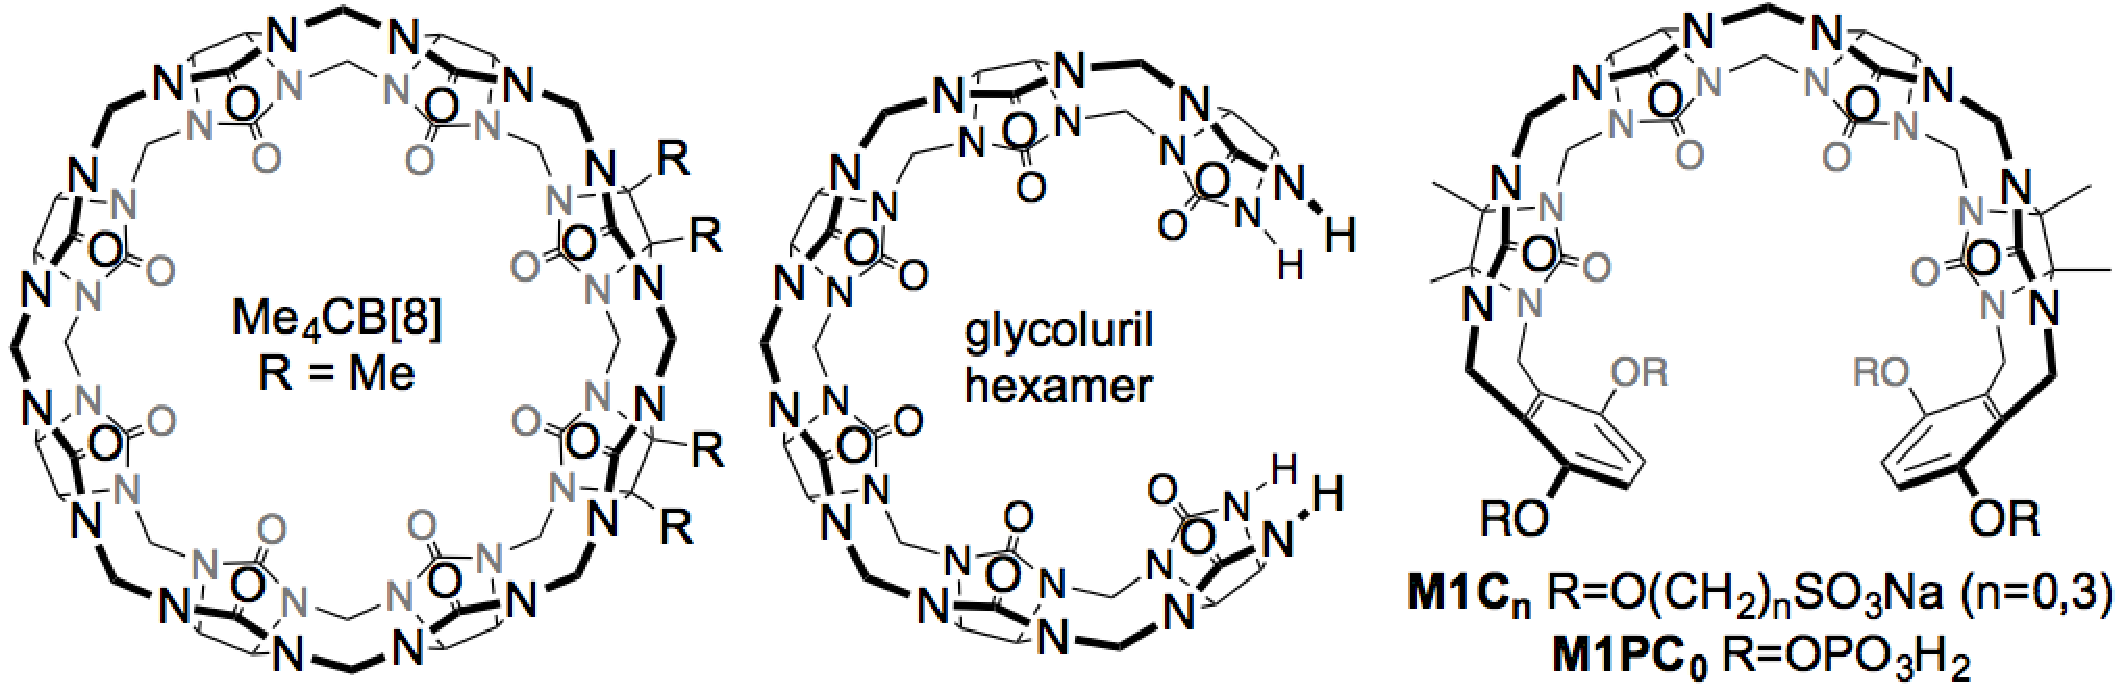
\includegraphics{figures/CB.pdf}}

\end{centering}

\vspace{0.1in}
\caption{\label{figure:CB} \footnotesize {\bf Structures of Me$_4$CB[8], glycouril hexamer, and acyclic CB[n]-type receptors.} These receptors bind a variety of drug-like molecules, some with high affinity, and this binding will form the basis of a cucubituril-based series of SAMPL binding challenges.}

\end{figure}

\textbf{SAMPL6, 8, and 10 cucurbituril challenges.} 
\emph{For SAMPL6}, we will measure $K_a$ and $\Delta H$ values, stoichiometry, and geometry for the interaction of Me$_4$CB[8] (a soluble CB[8] derivative) with 15 guests (selected top drugs, Table~\ref{table:CB}) by either direct or competition isothermal titration calorimetry (ITC), UV/Vis or fluorescence indicator displacement assay, or NMR competition experiments, as previously~\cite{cao_attomolar_2014, liu_cucurbituril_2005, ma_acyclic_2010, she_glycoluril-derived_2016}.  
Our selection of Me$_4$CB[8] binding to top drugs allows us to modulate the computational complexity by: 1) changing host flexibility (e.g. Me$_4$CB[8] can exhibit ellipsoidal deformation)~\cite{vinciguerra_synthesis_2015}, 2) allowing the possibility of binary or ternary (e.g. 1:1 and/or 1:2 host:guest) complexes~\cite{ko_supramolecular_2007, barrow_cucurbituril-based_2015, urbach_molecular_2011}, 3) using drugs with several potential binding epitopes to induce sampling issues.  Host:guest stoichiometry and geometry (e.g., which binding epitope is complexed) will be addressed by ITC $n$ values, Job plots monitored by UV/Vis or NMR~\cite{connors_binding_1987}, and by $^1$H NMR complexation induced changes in chemical shifts~\cite{masson_cucurbituril_2012}.  
All three sets of studies will be conducted in phosphate buffered saline (p$H$ 7.4 with physiological salt) which introduces its own complexities due to salt competition for binding~\cite{marquez_mechanism_2004, mobley_predicting_2016}. 
For \emph{SAMPL8}, we will focus on binding of the same 15 drugs (Table~\ref{table:CB}), but to glycoluril hexamer. 
This is an ideal next step as this host exhibits increased conformational dynamics, and influences the number and energy of solvating (and unusually coordinated) water molecules implicated in the high binding constants for CB[$n$]-guest complexes~\cite{biedermann_release_2012, biedermann_hydrophobic_2014}.  
The selected drugs include several with p$K_a$ values in the 3.8 to 7.4 range; given that CB[$n$]-type receptors (like biomolecular receptors) can induce pKa shifts in their guests of up to 4 pKa units~\cite{saleh_activation_2008, nau_deep_2011, ghosh_strategic_2012}, this will test how well models can predict these effects. 
Additionally, it will couple nicely with the focus on p$K_a$ values in Aim 1.
\emph{SAMPL10} will shift to acyclic CB[$n$]-type receptors (e.g. M1C$_3$, M1C$_0$, and M1PC$_0$ that contain anionic solubilizing groups attached via different linker lengths.  
As in SAMPL3~\cite{muddana_sampl3_2012}, these acyclic CB[$n$]-type receptors introduce conformational complexity, and water interactions play a key role.
Moreover, the presence of 4 anionic groups near the cavity will likely impact balance between ion-dipole interactions and the solvation of the free host.

{\bf Subaim 2.2. Gibb deep cavity cavitands for host-guest studies} 

%Gibb science

{\bf History of octa-acid SAMPL challenges.} During SAMPL4~\cite{gibb_binding_2013} and SAMPL5~\cite{sullivan_binding_2016} we focused on two hosts: the octa-acid 1 (R = H) and another octa-acid derivative with four methyl groups positioned at the portal of the binding pocket (1, R = Me). 
These studies used isothermal titration calorimetry (ITC) to measure the thermodynamics of (1) host {\bf 1} (R = H) complexing a range of 9 carboxylate guests,
and (2) the binding of 6 carboxylate and trimethylammonium guests to both hosts ({\bf 1}, H = H and Me; Figure~\ref{figure:gdccs}).  
In both cases $^1$H-NMR titration was also used to confirm ITC-derived free energies of binding.  
As noted above, co-solvent effects and water rearrangements posed particular challenges for predicting binding in these hosts. 
SAMPL5 emphasized how differences in the shape of the hydrophobic pocket of the host can have a profound affect on affinity for some guests~\cite{yin_overview_2016}.
% Comment on value to community


{\bf Novel deep cavity hosts probe the effects of binding site charge constellations.} 
For future SAMPL challenges, we will expand on the range of hosts by including {\bf 2} and {\bf 3} in our ITC studies (Figure~\ref{figure:gdccs}).  
Like cavitand {\bf 1}, host {\bf 2} is an octa-acid derivative.  However, the four benzoate groups are relocated from the extreme exterior in the case of {\bf 1}, to the rim of the binding pocket in {\bf 2}.  
We surmise that this will have a direct effect on the binding of charged guests, but more subtly, an indirect effect on guest complexation via changes to the solvation of the empty host.  
Octa-trimethylammonuim cavitand (``positand'' {\bf 3}) has the same overall architecture as host {\bf 1}, but inverts the charges on the water solubilizing exterior coat.  
While it is not yet clear if this switch in groups relatively remote from the pocket will directly affect guest complexation, results from related systems suggest it can (unpublished). 
Guests will be selected from commercial sources on the basis of reference calculations (on a larger set of guests) to ensure that they cover substantial dynamic range, marked differences in affinities between hosts, and/or affinities that depend substantially on the force field or water model, thus effectively testing our force fields and methods.

{\bf SAMPL6-10 deep cavity cavitand challenges.} 
The host-guest challenge for SAMPL6 will focus on how well the effect of host carboxylate substituent location can be predicted, and will involve hosts {\bf 1} and {\bf 2} with a set of five, previously uninvestigated guests.  
SAMPL7 will provide a second iteration of this experiment to test algorithmic improvements in predictive modeling following SAMPL6 by comparing hosts {\bf 1} and {\bf 3} with a different set of guests.  
We anticipate that because of the relative remoteness of the charged groups in these two hosts, the effects of switching charges will be subtler than the differences between {\bf 1} and {\bf 2}.  
SAMPL8 will consider the effect of common biologically-relevant counterions/salts salts on guest binding, comparing the effects of NaCl and NaI on the complexation of five guests to {\bf 1}.  
We have previously shown that iodide has a weak affinity for the binding pocket of {\bf 1}, whilst sodium ions have an affinity for the outer carboxylates~\cite{carnegie_anion_2014}, requiring modeling to capture the differential affinities of these ions in addition to guest affinities to successfully model the observed affinities.  
SAMPL9 will follow up on this by examining the effects of these same two salts on the complexation of five guests to {\bf 3}, again giving the modeling community time to incorporate algorithmic improvements following SAMPL8. 
While we have not yet quantified salt affinities to host {\bf 3}, we expect the iodide to have affinity for both the pocket and the positively charged solubilizing groups.  
For SAMPL10 we will consider the effects of co-solvents on the binding of five guests to {\bf 1} and {\bf 2} to probe the effect of co-solvent competition for the binding site, as well as effects cosolvents may have in weakening the hydrophobic effect. 
%* I'm a bit concerned that proposing to measure only five ligands per compound is going to be perceived as lacking in statistical power required to assess accuracy, and that this specific aspect will be a liability. Is it possible to do more than that, or would this require a significantly larger chunk of money or access to automated ITC technology? Alternatively, we can be vague about how many compounds we will use or focus on the total number of compounds across all hosts. (DLM: I should probably recast a bit somewhere to explain how much we'll learn across hosts. Here:)
While the number of guests considered in each challenge is relatively small, the total number of binding affinities measured is significant across the full family of hosts, meaning that the full data set will be of considerable value as a benchmark set~\cite{mobley_predicting_2016}. 

\begin{figure}[h]
\begin{centering}
\resizebox{\textwidth}{!}{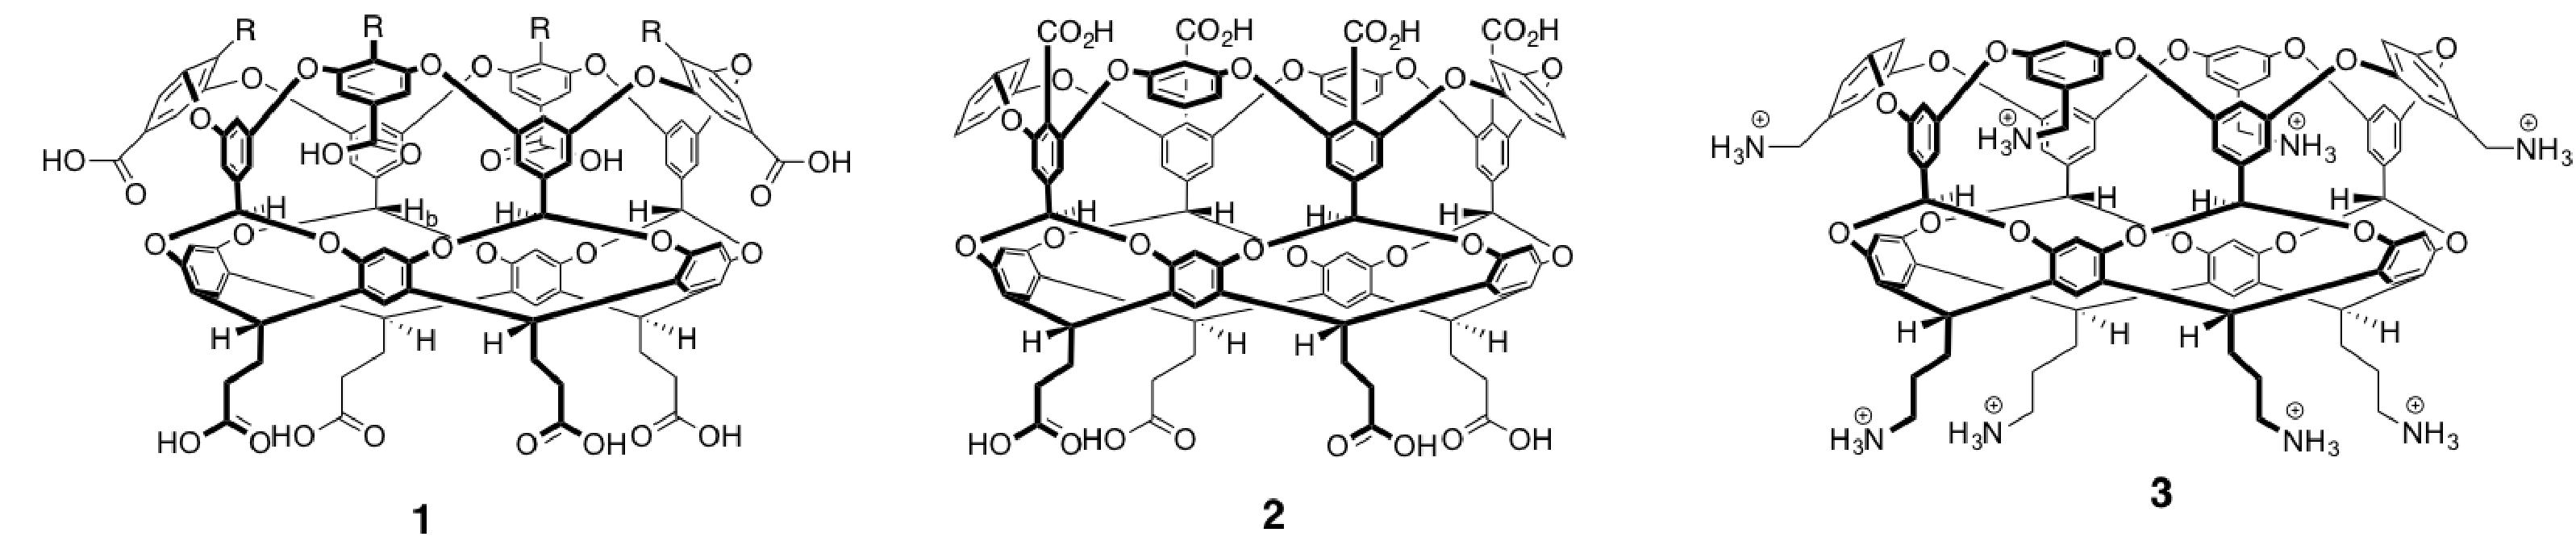
\includegraphics{figures/gdccs.pdf}}

\end{centering}

\vspace{0.1in}
\caption{\footnotesize {\bf Gibb deep cavity cavitands for SAMPL6-10.} These hosts bind a variety of carboxylate and trimethylammonium guests in a strongly salt-dependent manner, providing a stringent test of our ability to model binding and how it depends on these effects.
\label{figure:gdccs}}
\end{figure}


%Aim 3 - Generate biologically relevant advanced model systems for protein-ligand binding challenges. (2 pages) 
%{\bf Aim 3. Generate biologically relevant advanced model systems for protein-ligand binding challenges.}
\textbf{Aim 3: Develop model protein-ligand systems that isolate specific modeling challenges of drug targets.}
A major goal of our effort is to drive advances in the quantitative modeling of protein:ligand interactions.
While the Drug Design Data Resource (D3R~\cite{gathiaka_d3r_2016}) effort provides community blind challenges for biomolecular targets of pharmaceutical interest, these targets generally contain a daunting number of complexities that frustrate the ability for current methodologies to achieve quantitative accuracy, resulting in poor performance [CITE].
For example, while kinases are targets of great interest to drug discovery, blind challenges involving kinase targets conflate issues of slow protein conformational dynamics~\cite{Lin:2013:Proc.Natl.Acad.Sci.}, protonation state effects of both protein~\cite{Shan:2009:PNAS} and ligand~\cite{Szakacs:2005:JournalofMedicinalChemistry,Grante:2014:SpectrochimicaActaPartA:MolecularandBiomolecularSpectroscopy}, charged ligands, and the modeling of complex divalent salt environments and phosphorylation state effects along with the standard computational challenges of conformational sampling and forcefield accuracy.
While the value of these exercises as an accurate prospective benchmark of current-generation model accuracy is unquestionable, {\bf the ability of blind challenges on complex pharmaceutical targets to rapidly advance the field of quantitative predictive modeling is limited.}

Instead, {\bf our philosophy is to identify model protein:ligand systems with the goal of \emph{isolating} individual accuracy-limiting effects in iterative cycles of prospective blind community challenges.}
This process focuses the field on identifying and evaluating multiple solutions to the accuracy-limiting effects (such as how to deal with ligand and protein protonation-state issues~\cite{Onufriev:2013:QuarterlyReviewsofBiophysics}, slow protein conformational dynamics, etc.) free from other complicating factors, allowing a direct evaluation of how well the phenomena of interest are modeled.
Datasets collected for these blind challenges then become standard benchmark datasets for retrospectively examining the effectiveness of modeling approaches in treating these effects to facilitate comparisons of methodologies in publications, while future iterations or variations of the same SAMPL experiment allow iterative refinement and prospective blinded evaluations of methodologies.
In this way, this cycle of blind challenges utilizing model systems can rapidly drive progress in rapidly overcoming scientific hurdles limiting quantitative accuracy.

While model protein-ligand systems have a long and storied history of driving progress in individual research laboratories (such as the Shoichet T4 lysozyme mutants~\cite{merski_homologous_2015, mobley_predicting_2016}), their power in blind community challenge cycles is amplified by leveraging community participation.
An excellent example of this was the collection of a challenge dataset featuring the binding of small, rigid charged molecules to bovine trypsin for SAMPL3~\cite{Newman:2011:JComputAidedMolDes}, which rapidly focused the field on the deficiencies of current alchemical free energy methodologies in treating the binding of charged ligands.
Within two years, multiple laboratories had developed and disseminated convergent practical solutions to effectively handle charged ligand binding that are now adopted as best practices~\cite{Rocklin:2013:TheJournalofChemicalPhysics,Reif:2014:JournalofComputationalChemistry}.

{\bf SAMPL6-10 model protein:ligand challenges.} For the SAMPL6-10 challenges, we propose to introduce a new model protein:ligand system each year, with challenges fielded for each system for at least two consecutive years to allow iterative methodology improvement and assessment.
Immediately following the challenge, challenge data (including all primary data) will be published and released as a version-controlled benchmark dataset for retrospective evaluation.
The first challenge (introduced in SAMPL6) will focus on modeling the binding of small soluble drug fragments to a relatively rigid protein with multiple weak binding sites, isolating the ability of current-generation modeling approaches to model weak and multiple binding effects.
Because rapidly focusing the field on current challenges in predictive modeling requires the ability to adapt to deficiencies identified by D3R/SAMPL challenges of the previous year, subsequent model systems will be rapidly identified and developed using a new informatics platform we have developed to identify tractable model systems.

%%%%%%%%%%%%%%%%%%%%%%%%%%%%%%%%%%%%%%%%%%%%%%%%%%%%%%%%%%%%%%%%%%%%%%%%%%%%%%%%
% FIGURE: HSA SAMPL6 CHALLENGE
%%%%%%%%%%%%%%%%%%%%%%%%%%%%%%%%%%%%%%%%%%%%%%%%%%%%%%%%%%%%%%%%%%%%%%%%%%%%%%%%
\begin{figure}[h]
\begin{centering}
\resizebox{\textwidth}{!}{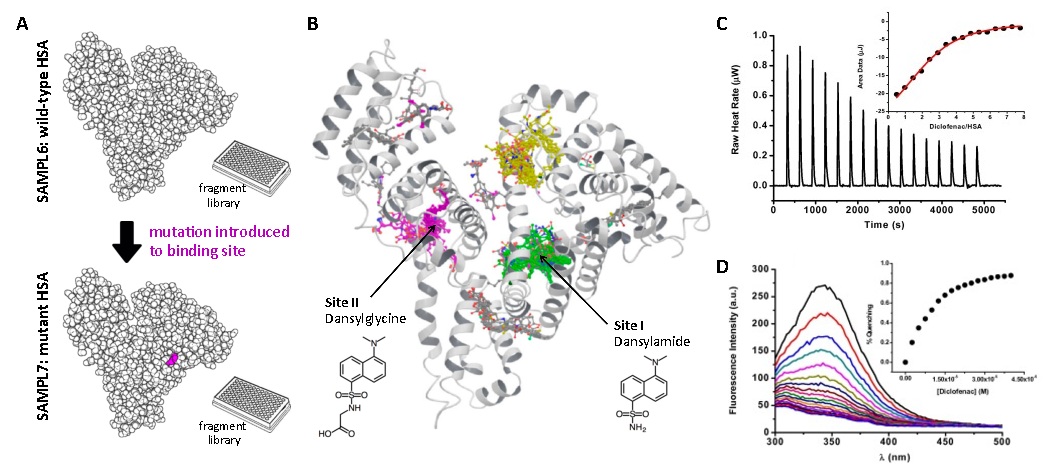
\includegraphics{figures/hsa-figure-draft4.pdf}}

\end{centering}
\vspace{0.1in}
\caption{\footnotesize {\bf The SAMPL6/7 protein:ligand challenge focuses on soluble drug fragment binding to human serum albumin (HSA).}
\emph{(A)}~SAMPL6 will introduce recombinant human serum albumin (HSA) as a target, against which a library of 96 small soluble drug fragments will be assayed.
By introducing a mutation in one of the binding pockets, we will create a second challenge target for SAMPL7.
\emph{(B)}~HSA, the most abundant plasma protein, has at least eight known binding sites, with major well-characterized sites (green, Sudlow's Site I; purple, Sudlow's Site II) observed to bind a variety of drugs, often modulating their pharmacokinetics~\cite{Fasano:2005:IUBMBLife(InternationalUnionofBiochemistryandMolecularBiology:Life)} (figure from~\cite{Hall:2013:JournalofChemicalInformationandModeling}).
Two fluorescent probes---dansylamide and dansylglycine---have been shown to bind with $\sim$$\mu$M affinity and high selectivity to Site I and Site II, respectively; both exhibit binding-enhanced fluorescence at 480 nm, and can be used to site-specifically probe ligand affinities by competition.
\emph{(C)}~Binding affinities of soluble molecules can easily be measured by isothermal titration calorimetry (ITC); here, the ITC titration of HSA by diclofenac (a Site II ligand~\cite{Rafols:2014:Talanta}) is shown~\cite{Bou-Abdallah:2016:TheJournalofChemicalThermodynamics}. 
\emph{(D)}~HSA tryptophan fluorescence quenching can also be used to measure ligand binding affinity; here, HSA titration by diclofenac is shown, with the inset plot showing percent quenching at 346 nm~\cite{Bou-Abdallah:2016:TheJournalofChemicalThermodynamics}
\label{figure:hsa-challenge}}
\end{figure}
%%%%%%%%%%%%%%%%%%%%%%%%%%%%%%%%%%%%%%%%%%%%%%%%%%%%%%%%%%%%%%%%%%%%%%%%%%%%%%%%

{\bf SAMPL6: Assessing predictive modeling to multiple weak binding sites with the binding of small soluble fragments to human serum albumin (HSA).}
Human serum albumin (HSA), the most abundant blood plasma protein, has the remarkable ability to bind a great variety of small molecule drugs in multiple binding sites (Figure~\ref{figure:hsa-challenge}B)~\cite{Fasano:2005:IUBMBLife(InternationalUnionofBiochemistryandMolecularBiology:Life)}.
As a result, HSA is not only an excellent model system for isolating the challenge of binding multiple weak ligands to a stable rigid protein, it is also a pharmacologically relevant system due to its ability to drastically modulate drug pharmacokinetics~\cite{Hall:2013:JournalofChemicalInformationandModeling}.
HSA has at least \emph{eight} known binding sites, with numerous crystal structures available for drugs binding to two predominant sites (Sudlow Site I and II)~\cite{Hall:2013:JournalofChemicalInformationandModeling}.
Small soluble molecules resembling drug fragments have previously been shown to have a high likelihood of detectable binding to HSA ($\ge$90\% of small druglike fragments, as detected by SPR~\cite{Elinder:2011:JournalofBiomolecularScreening}), providing an experimentally-tractable diverse set of ligands spanning several orders of magnitude in affinity [CITE].
As current advanced methodologies such as alchemical free energy calculations currently assume a single well-defined binding site with high affinity~\cite{Gilson:1997:BiophysicalJournal}, this dataset will allow the isolation of the effect of weak multiple binding from the majority of other counfounding factors in protein-ligand binding.

Recombinant HSA will be expressed in \emph{E.~coli} and purified via refolding from inclusion bodies~\cite{Latta:1987:Bio/Technology}, and will be defatted at low pH to ensure the resulting protein is free of the complications of both glycosylation and bound fatty acids found in plasma-isolated HSA~\cite{Lang:2015:BiotechnologyProgress}.
Recombinant expression will also allow a mutant form of HSA (engineered via quick-change single-primer mutagenesis) to be fielded for a SAMPL7 iteration of this challenge (Figure~\ref{figure:hsa-challenge}B).
We will obtain a diverse library of 96 soluble drug-fragment-like molecules in pre-plated format for which HSA-ligand affinities are not available in the literature as dry compound, and assay them for HSA binding using automated isothermal titration calorimetry (ITC) (Figure~\ref{figure:hsa-challenge}C), with the goal of characterizing the overall binding affinity of the compound to HSA.
%DLM: I'll have to edit the sentence above, as the adjective ("as dry compound") is very far separated from the noun (object) it modifies ("library"); also, the subject is singular ("library") but the second half of the sentence uses "them".
%If multiple binding events can be resolved, a multi-site model will be used; otherwise, a single dominant site will be assumed.
%Participants in the blind challenge will also have the option of predicting the ITC titration curve \emph{directly}, which includes all contributions to binding to multiple sites.
The same ligands pre-plated in DMSO format will be used to conduct a separate set of fluorescence titration assays (monitoring tryptophan fluorescence quenching) and competition assays in which the site-specific fluorescent probes daynsylamide (Site I) and dansylglycine (Site II) will be used to measure site-specific affinities for Sites I and II (Figure~\ref{figure:hsa-challenge}D), allowing participants to validate whether they predicted the correct binding site and, if so, the site-specific affinity.

{\bf SAMPL7-10: Rapid, responsive development of new model systems using a novel informatics platform.}
We have developed a novel informatics platform called TargetExplorer 
%[\url{https://github.com/choderalab/targetexplorer}] 
aimed at identifying new protein targets that can be rapidly developed into experimentally- and computationally-tractable model systems focusing on individual challenges.
This tool---which will be made accessible to other laboratories via an easy-to-use web interface during the course of this project---successively filters all protein:ligand complexes identified in the PDB according to a list of criteria that allow facile development as a model protein:ligand binding system, as well as identification of systems that isolate individual challenges in modeling accuracy.
Experimental tractability includes: (1) the availability of multiple protein:ligand crystal structures; (2) known bacterial expression (e.g.~from PDB {\tt EXPRESSION\_SYSTEM} records); (3) the capacity to bind a wide dynamic range of ligands (determined via data available in ChEMBL); (4) the availability of multiple known ligands that can be purchased (via ZINC); (5) tractability of experimental affinity measurements, such as known ligands with potentially fluorescent scaffolds (for fluorescence competition assays), highly soluble ligands (for ITC), or ligands above a minimal mass (for SPR or MST).
A number of additional filters annotate potential experimentally tractable systems for suitability as a model system that isolates individual challenges, such as: charged ligands or potential ligand protonation state or tautomer~\cite{Martin:2009:JournalofComputer-AidedMolecularDesign} effects (deduced from predicted aqueous protonation/tautomer energies); potential protein protonation state effects (deduced from MCCE2 calculations~\cite{Song:2009:JournalofComputationalChemistry}); protein conformational changes (deduced from variation in protein conformation or the presence of unresolved loops in protein:ligand crystal structures); the presence of post-translational modifications that may affect affinity (deduced from Uniprot annotations); coordinated metals (identified in crystal structures); ordered waters (present in multiple crystal structures); etc.

The Chodera lab has developed an automated wetlab for the purpose of rapidly developing model protein systems using bacterial expression techniques (see Equipment and Facilities).
Potential targets matching desired challenge criteria will be screened for bacterial expression using high-throughput cloning, transformation, and expression testing, with purity and yield assessed by capillary electrophoresis on a Caliper GXII.
Targets will be screened for stability in various buffers using Thermofluor~\cite{Reinhard:2013:ActaCrystallographicaSectionFStructuralBiologyandCrystallizationCommunications}.
Ligands identified via the informatics platform to span a wide dynamic range of binding affinities will be purchased as dry powder stocks and prepared for assay by highly accurate gravimetric solution preparation techniques using a Quantos automated balance.
A wide variety of biophysical techniques are available to provide accurate, quantitative measurements of protein-ligand binding affinities, including fluorescence (if fluorescent probe ligands are available), absorption (e.g.~Soret band shifts), automated isothermal titration calorimetry (provided ligands are sufficiently soluble), surface plasmon resonance, microscale thermophoresis (MST), luminescence, and alphascreen; all except MST are fully automated.

Our approach to developing challenge datasets will be twofold:
First, small molecules similar to known ligands will be purchased and assayed, with the presumption that these molecules are likely to have measurable affinities.
Second, site-directed mutants will be introduced to modulate the binding affinities of known ligands using single-primer quick-change mutagenesis, which can be performed and screened for expression in 96-well format.
Challenge datasets will therefore consist of a matrix of protein mutants and ligands, providing a rich dataset to deeply explore the effects of interest.

%We will identify suitable biological protein-ligand model systems (difficult but tractable in order to push the limits of physical techniques) then measure binding and develop these for blind challenges. This will include binding studies on human serum albumin and bromodomains or aspartyl proteases; initial binding data will be expanded by the selection of additional ligands or the creation of mutations in the protein that modulate binding.

%%%%%%%%%%%%%%%%%%%%%%%%%%%%%%%%%%%%%%%%%%%%%%%%%%%%%%%%%%%%%%%%%%%%%%%%%%%%%%%%
% FIGURE: MODEL SYSTEM MINING
%%%%%%%%%%%%%%%%%%%%%%%%%%%%%%%%%%%%%%%%%%%%%%%%%%%%%%%%%%%%%%%%%%%%%%%%%%%%%%%%
\begin{figure}[h]
\begin{centering}
\resizebox{!}{2in}{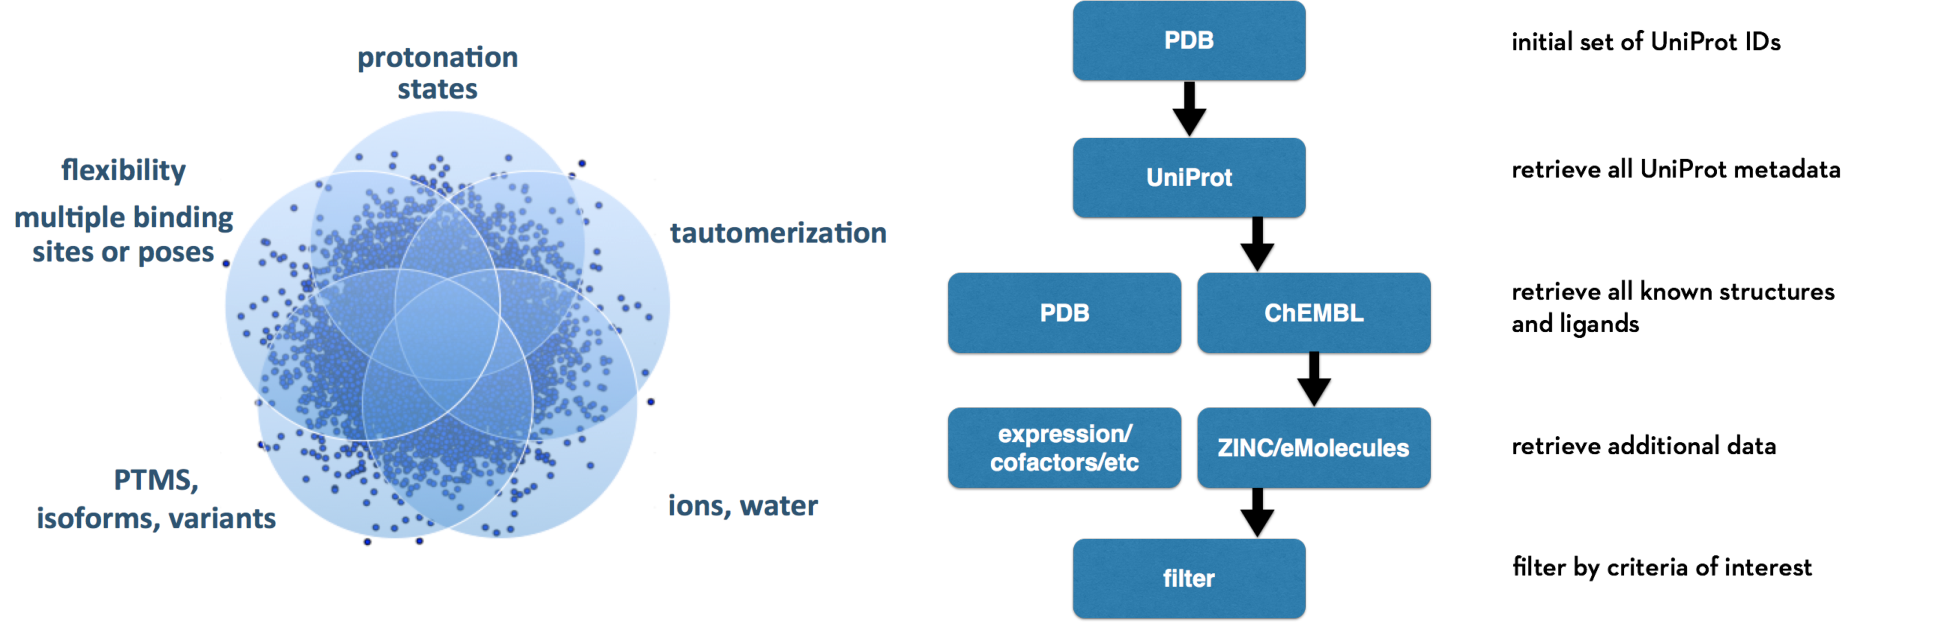
\includegraphics{figures/mining-model-systems.pdf}}

\end{centering}
\vspace{0.1in}
\caption{\footnotesize {\bf Mining model protein:ligand systems to focus on individual modeling challenges via a structural and chemical informatics platform.}
SAMPL7-10 will feature the introduction of new model protein:ligand systems designed to focus on individual challenges judged to be of critical immediate importance following current D3R/SAMPL blind competitions.
\emph{Left:} Since most protein targets of pharmaceutical interest feature a multitude of conflated challenges to quantitative accuracy, our goal is to identify model protein targets that isolate individual effects to focus community efforts by fielding new blind challenges.
\emph{Right:} In order to rapidly develop new experimentally- and computationally-tractable model protein:ligand systems, we have developed a structural and chemical informatics system that applies successive filters to the set of \emph{all} potential protein:ligand systems for which structural data is available.
{\color{red}[JDC: This figure is a placeholder.]}
\label{figure:mining-for-model-systems}}
\end{figure}
%%%%%%%%%%%%%%%%%%%%%%%%%%%%%%%%%%%%%%%%%%%%%%%%%%%%%%%%%%%%%%%%%%%%%%%%%%%%%%%%



%Aim 4 - Coordinate, run, and analyze blind challenges to advance modeling of binding (1.5 pages)
{\bf Aim 4: Field iterated community blind challenges to advance quantitative biomolecular design.}
While the data generated in Aims 1-3 is valuable in its own right, \textbf{the real impact of this work comes from using this data to conduct regular SAMPL blind challenges} which test the state of the art, drive new methodological and force field innovations, allow comparative evaluation of methods, and result in downstream improvements.
The new, progressive nature of the data generated for SAMPL6-10 means that these challenges will build on one another, and for success in later SAMPL challenges, participants must build on lessons learned from prior challenges.
SAMPL challenges will thus serve to guide improvements to quantitative modeling of binding, facilitating regular cycles of application, learning, and improvement of models.

% I didn't have this in the outline (bizarrely) but we need to briefly explain how we actually run a SAMPL challenge:
SAMPL challenges will have submission deadlines yearly, though not every data type or component of Aims 1-3 will be annual.
The full timeline for SAMPL challenges (below) will be made available on the SAMPL website (https://drugdesigndata.org/about/sampl) when this project begins, allowing participants to plan their work and select what challenges to be involved in.
As experimental data for each component becomes available and is curated, input files and challenge details will be made available online (and we will advertise via our e-mail list from prior SAMPLs and CCL), at least six months prior to the challenge deadline; data not yet available at that time will be held for a subsequent challenge.
The exception will be in Year 1 of the project where, due to startup timescales, we expect to only be able to allow 3 months. 
%Some of the timing details here could be bumped to Timeline I think [DLM]
As in prior SAMPLs, submissions will be handled by an automated web upload service on the SAMPL website (which will be migrated to separate hosting if the D3R effort is not renewed after its current term) which pre-processes submissions to ensure that they meet format standards we specify along with the challenge details. 
These format specifications ensure predictions can be automatically handled by our Python analysis framework.
As in SAMPL4 and SAMPL5, analysis will also be conducted by our automated Python framework, as will e-mail return of plots and data analysis associated with each submission.
As usual, participants will be allowed to submit multiple sets of predictions per SAMPL component to allow for comparative assessment of models.
One new ingredient will be that each participant will be required to designate one submission as their ``primary'' submission which will be included in the formal ranking of performance; other submissions will still be analyzed and receive an assessment of performance, but only one will be formally ranked.
We find that participants learn a great deal from being able to compare multiple methods or protocols, but providing some participants with more ``shots on goal'' than others in the formal ranking can be seen by some as unfair.
%The above two sentences can probably be cut if we are tight on space.
As previously, we will continue making all participant submissions and method descriptions available publicly on the website, along with author information except with authors specifically request to remain anonymous prior to submission.

%Coordinate and run SAMPL blind challenges
\textbf{Our goal in this aim is not just to run blind challenges, but to advance modeling by helping participants understand where they went wrong, why, and how they might do better next time}. 
To achieve this, we provide guidance to participants as to what challenges we expect may be important when we provide details on each SAMPL component.
For a host-guest system, for example, we might highlight known buffer/salt effects, protonation state challenges, and point out previous work on sampling challenges, with pointers to the relevant experimental work and to modeling work from past SAMPL challenges and elsewhere (i.e. as in \cite{mobley_predicting_2016}).
This helps participants design their approach.
%Run reference calculations to:
Additionally, we find it important to run reference calculations of our own to explore various approaches. This serves several purposes:
		%a. Test current standard methods/FF
It provides a test of the current methods we select (usually those we view as current standard best practices) and current force fields; 
		%b. Facilitate others learning (swap method or FF)
it helps facilitate learning -- we announce what calculations we plan to perform, make input files available in a wide variety of formats [ref HG, DC overviews and Shirts], and others can repeat our calculations with a different method but same system and force field to compare methods, or swap force field but keep the method and system fixed to compare force fields, etc.; 
		%c. Do sensitivity analysis (learn what?s important)
and it allows us to conduct sensitivity analysis, as by varying the conditions of our simulations (protonation state, tautomer, etc.~\cite{bannan_blind_2016}) we can see how much this impacts calculated values and thereby how important it is, even if participants don't do these tests.
		%d. (Give examples of what we've learned from this)
Reference calculations have, for example, helped us highlight the importance of a small amount of water in cyclohexane for accurately calculating log D values, determine that an incorrect tautomer could affect calculated values by many log units~\cite{bannan_blind_2016}, and highlight how forcefield modifications could significantly improve results on hydration free energies~\cite{mobley_blind_2014-1}.
		%e. (We will make inputs, outputs, and methods available too)
To further aid follow up studies, we will make the input files, results, and even simulation methods used for our reference calculations along with the calculations themselves, with the methods being made available via our open software development efforts on GitHub.


%Select and announce null models, run them
Physical methods are only valuable if they can reliably outperform alternate methods, so \textbf{a new focus of SAMPL6-10 will be selecting quality null models and running them to provide a point of comparison for participants}.
While SAMPL efforts in the past have used some null models, lack of manpower has required that these be particularly crude (such as ``guess zero'' models [refs]) which provide no predictive value. 
In this work, we will announce our selected null models when we open each challenge component, so participants know what their results will be compared with.
%Do statistical analysis of results (& compare to nulls), report back
Statistical analysis of SAMPL performance, and comparison with nulls, will continue to be an important component of our work [refs].

%D3R coordination/meetings:
Following submission and analysis of each SAMPL challenge, challenge results will be released and discussed, with SAMPL workshops allowing more formal presentations on and discussion of results in years 1, 3, and 5. 
	%	a. Co-running workshops with D3R
Workshops will run every two years at the request of past participants, and will be co-run and co-hosted with D3R Grand Challenge workshops (see support letter).
During the off years, SAMPL challenges will still run, but discussion of and dissemination of results will be via asynchronous means (as discussed below) and a ``virtual workshop'' consisting of talks and interaction over Google Hangouts or YouTube Live (formerly Hangouts On Air).
	%     b. Coordinating challenges with them, submission deadlines offset from D3R challenges
While coordination with D3R will mostly be at the level of workshops, we will also work with them ensure that SAMPL challenge submission deadlines are offset from deadlines for D3R to allow maximum community participation in both efforts.

	%Coordinate with JCAMD on special issues
Dissemination of results is particularly key so that new insights can be rapidly spread to the community.
We will continue to work with JCAMD to publish regular SAMPL special issues (see support letter), but timescales for this can be slow.
	%Encourage prepublication sharing (bioRxiv) and sharing of slides/posters (F1000?)
Therefore, we will strongly encourage prepublication sharing of results and analysis, most immediately via sharing of slides and posters such as via F1000 Research and then paper preprints via bioRxiv or similar.
	%Provide a way to connect up researchers to enable rapid progress, such as Slack
We also want to ensure that participants are able to learn from one another via exchanging ideas outside of formal workshops and meetings.
While this has happened in the past -- for example, when workers whose methods should yield identical results find differences, they often work together to identify the origin of these discrepancies [refs] -- it often occurs only between isolated individuals.
To facilitate more open communication between the community, we will make a SAMPL group on the Slack collaboration software, with channels corresponding to each component of each challenge, allowing interested individuals to openly exchange ideas, tests, and work together to learn from their work.

	%Data curation, archival and dissemination
\textbf{Each data set naturally should undergo a life cycle of collection, curation, blind challenges, and public dissemination}.
In the past, SAMPL has primarily emphasized the \emph{blind challenges} and pre-challenge \emph{curation} aspects, with isolated forays into collection [ref SAMPL5, ref Peat trypsin]. 
This work considers the full life cycle for the first time, with Aims 1-3 dealing primarily with collection and pre-challenge curation.
Post-challenge, 
	%   Datasets will be curated and released as standard community benchmark datasets: For example, FreeSolv
datasets will receive additional curation and then be released to the community as standard test or benchmark sets [ref benchmark set paper]. 
One related example of such a set is the FreeSolv dataset, which includes a large number of calculated and experimental hydration free energies, including those from SAMPL0-SAMPL4 [ref].
	%   Data curation also via follow-up experiments (new!; cite examples where it was desirable)
Post-challenge curation will also receive new attention here; in the past, lack of resources has always prevented follow-up experimental work, even when the data clearly indicated it was warranted (such as puzzling issues with dynamic range for log D values in SAMPL5 [ref]).
These experiments will now be conducted, allowing computation to drive collection of additional experimental data when warranted.
	%   Store and archive primary data and analysis
Dissemination is the final stage in the data life cycle; we discuss how exactly the data will be disseminated in more detail in our Resource Sharing plan, but essentially, we will make the data (including primary data, processed data, and our analysis of challenge submissions) available freely and publicly with permanent, cite-able DOIs, and with backup hosting on library facilities (such as UCI's DASH [link]) to ensure availability long after termination of the project.
Binding data will also be deposited in BindingDB [ref].

	%   Probably also should comment on archiving/disseminating OLD SAMPL data, which we haven't been able to do (lack of resources)
Because prior SAMPL work focused mainly on challenges themselves, dissemination of the data has never been a major focus.
As part of this project, we will retrieve old SAMPL experimental data, submissions, and analysis from where it is archived and make it available along with the new data generated here. 

	%   Methodology archival? Push for containerization of tools, maybe in conjunction with other known efforts. [Currently short on space, but putting something very short on this here anyway.]
We will also push for containerization of tools and methods in conjunction with other efforts such as AutoDesk's Molecular Design Toolkit and the NSF Molecular Sciences (MolSci) initiative.
Our vision is that long-term, instead of participants submitting a set of predictions, they would also submit the entire workflow they applied via Docker containers in a way which would allow others to reproduce their work if needed, or to repurpose the workflow for new applications, ensuring not just that SAMPL \emph{results} get disseminated, but that the \emph{methods} and \emph{workflows} themselves spread.


%%%%%%%%%%%%%%%%%%%%%%%%%%%%%%%%%%%%%%%%%%%%%%%%%%%%%%%%%%%%%%%%%%%%%%%%%%%%%%%%%%%%%%%%%%%%%%%%%%%%%%
% TIMELINE
%%%%%%%%%%%%%%%%%%%%%%%%%%%%%%%%%%%%%%%%%%%%%%%%%%%%%%%%%%%%%%%%%%%%%%%%%%%%%%%%%%%%%%%%%%%%%%%%%%%%%%

{\bf \large TIMELINE} %1 page minus a paragraph (CURRENTLY THIS IS TOO LONG).
%"The timeline is actually likely to be very important here, so I'd strongly suggest we include it, if not expand it to one full page. We have to "sell" the reviewers on how the concept would play out into actual challenges, advances, etc. so that they get a concrete idea of all the good things that will come of this. We should mention when we would hold blind challenges, when data would be released, when meetings would occur, when benchmarks would be published, and what datasets would be generated for the community."
{\color{red}[Insert a 0.25-page figure to summarize SAMPL iterations and coordinated challenges in each category (Aim 1, Aim 2, Aim 3).]}


\textbf{Yearly challenges will drive progress.}
{\color{red}[DLM: This has a lot of overlap with Aim 4 in terms of what timing details it gives, so I'll have to shrink one or the other to remove redundancy.]}
Our series of SAMPL challenges is progressive in difficulty, with subsequent challenges building on those from previous years and driving progress towards biomolecular binding for pharmaceutical datasets as covered by D3R.
%Will have to update language here to distinguish whether we're going with the "one deadline a year" model or the "rolling deadlines"/"staggered deadlines" model
Each year's SAMPL challenge involves several components with staggered deadlines set to maximize scientific benefit. 
Tentative deadlines and the full project Timeline (Figure X) will be made available as soon as the project kicks off in order to allow workers to plan.
Inputs will be available on our website at least 6 months prior to the challenge deadline (except in the first year, when data collection will require a more limited window of 3 months).
Automated analysis of submissions -- which are required to be in a standard format -- will already be online prior to the submission deadline, so immediately following the deadline, participants will receive automated reports giving the experimental results, a detailed summary of the statistics for each of their submissions and how they compare to other methods. 
This will also include distribution of the method descriptions that participants submit along with their predictions, allowing challenge participants to see how top performing methods differed from their own approaches.
Results from our reference calculations will also be distributed at the same time.
At this time participants will also receive information directing them to Slack channels (see above) for discussion of the challenge and results, as well as publication information.

\textbf{Follow-up information exchange facilitates improvements.}
Immediately following return of challenge results, follow up communication on Slack channels focused on each challenge component will spur participants to share what they did, what they learned from it, and begin learning from one another and from us and our reference calculations.
Normally, challenge participants have explored different aspects of the challenge, with some looking at details of convergence, others comparing force fields and water models, and so on. 
Often, this information only comes out only in publication, long after the challenge deadline and any meetings which might result.
Our vision is to use the more rapid conversation that comes via Slack to propagate this information earlier. 
Individual messages in Slack have permanent links, meaning that participants who share here will have a permanent record of their contribution to the science -- reducing concerns that ideas shared pre-publication might not receive credit. 
This will be the primary means of communication regarding SAMPL for eight weeks after the challenge deadline.
After this eight week period, a virtual meeting will wrap up the particular challenge component and allow participants to begin refocusing their efforts on the next challenge, with ten months until the next deadline for that component and four months until the data becomes available. 
This will provide enough time to incorporate lessons learned.
Overall meetings -- virtual (years 2 and 4) or in-person (the end of years 1, 3, and 5) will wrap up the overall challenge; these will be timed to follow the last component challenge of each of the relevant years.
%Writing this now that the budget is finalized, realizing that it would have been better to say overall meetings in year 2, early in year 4, and end of year 5, as end of year 1 is too early. But, can't change that now, so we can just deal with it when we re-budget after they cut the budget... 

\textbf{Publication reaches a broader audience.}
During the initial eight weeks after the submission deadline/return of results, participants will be encouraged to begin preparing their results for publication.
We highly encourage the use of preprints to get material out to the broader audience as quickly as possible.
However, as noted, we will continue to work with JCAMD to have regular special issues focused on SAMPL. 
Deadlines for these will be yearly, and the review/revision process is normally expected to take around two months from submission until when papers begin appearing online. 
Composition of the special issue itself has to take longer, as the issue can't be finalized until all papers are typeset. 
Thus our priority, for rapid dissemination is on more rapid means of communication, though the permanent academic record of the work will continue to need to be traditional publishing.


\textbf{Datasets generate lasting value as benchmarks.}
As discussed in Aim 4, all SAMPL data will be made easily and publicly available to serve the community in the future as retrospective tests, and will be deposited in standard repositories such as BindingDB when applicable.
In some cases, the cumulative value of data will be profound. 
For example, some of the host-guest challenges do not incorporate a particularly large number of compounds, but over the lifespan of SAMPL6-10, the amount of data accumulated will be considerable.
Selected SAMPL data sets are expected to become especially valuable as standard benchmark sets and will receive additional attention by being singled out by the community as such~\cite{mobley_predicting_2016}.
In these ways, SAMPL will have a lasting effect on the modeling community.

%%%%%%%%%%%%%%%%%%%%%%%%%%%%%%%%%%%%%%%%%%%%%%%%%%%%%%%%%%%%%%%%%%%%%%%%%%%%%%%%
% FIGURE: AIMS OVERVIEW
%%%%%%%%%%%%%%%%%%%%%%%%%%%%%%%%%%%%%%%%%%%%%%%%%%%%%%%%%%%%%%%%%%%%%%%%%%%%%%%%
%\begin{figure}[h]
%\begin{centering}
%\resizebox{\textwidth}{!}{\includegraphics{figures/timeline.pdf}}

%\end{centering}
%\vspace{0.1in}
%\caption{\footnotesize {\bf Timeline.}
%\label{figure:aims-overview}}
%\end{figure}
%%%%%%%%%%%%%%%%%%%%%%%%%%%%%%%%%%%%%%%%%%%%%%%%%%%%%%%%%%%%%%%%%%%%%%%%%%%%%%%%

%%%%%%%%%%%%%%%%%%%%%%%%%%%%%%%%%%%%%%%%%%%%%%%%%%%%%%%%%%%%%%%%%%%%%%%%%%%%%%%%%%%%%%%%%%%%%%%%%%%%%%
% COLLABORATION MANAGEMENT PLAN
%%%%%%%%%%%%%%%%%%%%%%%%%%%%%%%%%%%%%%%%%%%%%%%%%%%%%%%%%%%%%%%%%%%%%%%%%%%%%%%%%%%%%%%%%%%%%%%%%%%%%%

{\large \bf COLLABORATION MANAGEMENT PLAN} % 1 paragraph
% Collaboration history of success: Mobley and Chodera have worked together extensively in past SAMPL challenges and other areas; Mobley/Isaacs and Mobley/Gibbs have fielded past SAMPL challenges.
% PI Mobley will oversee entire project; Mobley/Chodera A1, Isaacs SA 2.1, Gibb 2.2, Chodera A3, Mobley/Chodera A4 (tapping other co-I as needed).
% How often will PI and co-Is talk/meet?
% Publication management plan.
% Conflict resolution plan.

We have a strong previous history of successful collaboration, with Mobley and Chodera having co-authored roughly a dozen publications since 2006, as well as several workshops and other initiatives.
Mobley, Isaacs, and Gibb have also worked together to coordinate past SAMPL challenges, and Mobley and Gibb a previous NSF workshop. 
PI Mobley will oversee the entire project, with Mobley and Chodera working together on Aim 1 (Mobley working with west coast pharma; Chodera with east coast), Isaacs responsible for Aim 2.1, Gibb for Aim 2.2, and Chodera for Aim 3. Mobley and Chodera will conduct aim 4, involving the other co-investigators as needed.
Meetings will consist of a Google Hangout monthly and an in-purpose planning meeting once yearly which will take place at the SAMPL workshops during the years those are offered, and a separate meeting doing the alternate two years.
Chodera and Mobley will communicate more frequently due to the interlinked nature of their work.
Publications are expected to be largely dictated by the overall Timeline noted above, with an experimental publication associated with each challenge component being prepared for distribution to participants along with their results.
Conflict resolution is expected to be straightforward given the extensive past history of interaction and collaboration between the investigators, but if any serious difficulties arise, Michael Gilson (UCSD) will be consulted as an arbiter, given the need this initiative has for close connections with D3R.

{\large \bf OUTLOOK} %or conclusions. 0.5 page
% This part is probably less critical, and can be dropped if space reasons dictate.

Physical methods have been slow to achieve their promise in binding prediction, in part because truly significant innovations are so hard to recognize due to a lack of standard tests and benchmarks, and in part because of an ``applications first'' approach which seems to plague our community where we rush to apply our methods to problems of pharmaceutical relevance without ensuring they can tackle simpler, better-understood problems first.
Here, we propose an innovative extension of the successful series of SAMPL blind challenges, generating novel experimental data to drive improvement of the methods in our field and help them become pharmaceutically relevant -- beginning with relatively simple physical property prediction and progressing to challenging problems in biomolecular recognition via a series of carefully designed intermediate steps.
SAMPL already has a strong track record of success, and funding will ensure an even greater impact on the community and that it is around as a valuable resource for years to come.
The proposed series of carefully tailored challenges will focus our community on a variety of problems which we \emph{can} realistically resolve in the near term, resulting in dramatic improvements in the field's ability to do computational molecular design.

%%%%%%%%%%%%%%%%%%%%%%%%%%%%%%%%%%%%%%%%%%%%%%%%%%%%%%%%%%%%%%%%%%%%%%%%%%%%%%%%%%%%%%%%%%%%%%%%%%%%%%
% BIBLIOGRAPHY
%%%%%%%%%%%%%%%%%%%%%%%%%%%%%%%%%%%%%%%%%%%%%%%%%%%%%%%%%%%%%%%%%%%%%%%%%%%%%%%%%%%%%%%%%%%%%%%%%%%%%%

\eject

%\footnotesize
%\scriptsize
%\bibliographystyle{acm}
\bibliographystyle{nci}
%\bibliographystyle{nar}
\bibliography{sampl-r01}

\end{document}